\usetikzlibrary{
  calc, 
  intersections, 
  arrows,
  patterns,
  angles,
  quotes,
  decorations,
  babel,
  fadings
}
% \usetikzlibrary{qrr.arc}

%Styles
\tikzset{
dot/.style={circle, fill=black, inner sep=1.5pt}
}
\tikzset{
winkel/.style={draw=black,angle radius=1cm}
}
\tikzset{
winkelsmall/.style={draw=black,angle radius=.6cm}
}

\tikzset{
>=latex
}


\newcommand*\savepos[1]{% 
	\tikz[remember picture,baseline=(#1.base)]\node[inner sep=0pt](#1){\strut};% 
} 
\newcommand*\pright[4][0.8,0]{% 
	\tikz[remember picture,overlay]% 
	\draw[very thick,->](#2).. controls +(#1) and +(#1) ..(#3)node[midway,right]{#4};}

\newcommand*\pleft[4][-0.8,0]{% 
	\tikz[remember picture,overlay]% 
	\draw[very thick,->](#2).. controls +(#1) and +(#1) ..(#3)node[midway,left]{#4};}


%%%%%%%%%%%%%%%%%%%%%%%%%%%%%%%%Mekruphy%%%%%%%%%%%%%%%%%%%%%%%%%%%%%%%%
\newcommand{\platte}{
	\draw[very thick] (0,0) rectangle (11,11);
	\draw[very thick] (1,4) -- ++(0,-1) -- ++(3,0) -- ++(0,2) ++ (0,-2) -- ++(0,-2) ++ (0,2) ++ (3,0) -- ++(0,2) ++ (0,-2) -- ++(0,-2) ++ (0,2) -- ++(3,0) -- ++(0,1) ++ (0,3) -- ++(0,3) -- ++(-1,0) ++ (-1,0) -- ++(-1,0) ++ (-3,0) -- ++(-1,0) ++ (-1,0) -- ++(-1,0) -- ++(0,-3);
	\foreach \x/\y in {1/4,1/7,2/10,3/10,4/1,4/3,4/5,4/10,7/1,7/3,7/5,7/10,8/10,9/10,10/7,10/4}
	\draw[fill=white,very thick] (\x,\y) circle [radius=2mm];
}

%%%%%%%%%%%%%%%%%%%%%%%% Grosse Symbole %%%%%%%%%%%%%%%%%%%%%%%%%%%%%%%
\newcommand{\xllampe}[3]{
	\fill (#1,#2) circle [radius=2mm];
	\fill (#1+#3,#2) circle [radius=2mm];
	\draw[very thick] (#1,#2) to [bulb, huge circuit symbols] ++(#3,0);
}

\newcommand{\xlbatterie}[3]{
	\fill (#1,#2) circle [radius=2mm];
	\fill (#1+#3,#2) circle [radius=2mm];
	\draw[very thick] (#1,#2) to [battery={name={Bat1}}, huge circuit symbols] ++(#3,0);
	\node at (Bat1) [above=3.5mm,left] {+};
	\node at (Bat1) [above=3mm,right] {-};
}

\newcommand{\xlvoltmeter}[3]{
	\fill (#1,#2) circle [radius=2mm];
	\fill (#1+#3,#2) circle [radius=2mm]; 
	\draw[very thick] (#1,#2) to [voltmeter,huge circuit symbols] ++ (#3,0);
}

\newcommand{\xlamperemeter}[3]{
	\fill (#1,#2) circle [radius=2mm];
	\fill (#1+#3,#2) circle [radius=2mm]; 
	\draw[very thick] (#1,#2) to [ammeter,huge circuit symbols] ++ (#3,0);
}

\newcommand{\xlschalter}[3]{
	\fill (#1,#2) circle [radius=2mm];
	\fill (#1+#3,#2) circle [radius=2mm]; 
	\draw[very thick] (#1,#2) to [make contact,huge circuit symbols] ++ (#3,0);
}

%%%%%%%%%%%%%%%%%%%%%%%%%%% Kleine Symbole %%%%%%%%%%%%%%%%%%%%%%%%%%%%%%%%%

\newcommand{\lampe}[3]{
	\fill (#1,#2) circle [radius=2mm];
	\fill (#1+#3,#2) circle [radius=2mm];
	\draw[very thick] (#1,#2) to [bulb] ++(#3,0);
}

\newcommand{\batterie}[3]{
	\fill (#1,#2) circle [radius=2mm];
	\fill (#1+#3,#2) circle [radius=2mm];
	\draw[very thick] (#1,#2) to [battery={name={Bat1}}] ++(#3,0);
	\node at (Bat1) [above=3.5mm,left] {+};
	\node at (Bat1) [above=3mm,right] {-};
}

\newcommand{\voltmeter}[3]{
	\fill (#1,#2) circle [radius=2mm];
	\fill (#1+#3,#2) circle [radius=2mm]; 
	\draw[very thick] (#1,#2) to [voltmeter] ++ (#3,0);
}

\newcommand{\amperemeter}[3]{
	\fill (#1,#2) circle [radius=2mm];
	\fill (#1+#3,#2) circle [radius=2mm]; 
	\draw[very thick] (#1,#2) to [ammeter] ++ (#3,0);
}

\newcommand{\schalter}[3]{
	\fill (#1,#2) circle [radius=2mm];
	\fill (#1+#3,#2) circle [radius=2mm]; 
	\draw[very thick] (#1,#2) to [make contact] ++ (#3,0);
}

\newcommand{\kasten}[1]{
	\draw (0,0) coordinate (A) rectangle ++(2.5,1) coordinate (B);
	\node at ($.5*(A) + .5*(B)$) {#1};
}

\newcommand{\achtung}[1]{
\begin{minipage}{2.5 cm}

\begin{tikzpicture}[scale=0.5]
 \draw[rounded corners=4pt, fill=black] (0,0) -- (4,0) -- (2,3.464) -- cycle;
 \draw[rounded corners=4pt, fill=white] (0.5,0.289) -- (3.5,0.289) -- (2,2.964) -- cycle;
 \draw[fill=black] (2,0.6) circle [radius=1mm];
 \draw[fill=black] (1.9,1) to [out=270, in=270] (2.1,1) -- (2.2,2.3) to [out=90, in=90] (1.8,2.3) -- cycle;
\end{tikzpicture}
\end{minipage}
\vspace{0.5cm}
\begin{minipage}{16cm}
 #1
\end{minipage}

}

\newcommand{\karo}[2]{
\begin{tikzpicture}
\draw[step=.5cm, very thin] (0.1cm,0.1cm) grid (#1-0.1,#2-0.1);
\end{tikzpicture}
}

\newcommand{\tikzkaro}[5][thin]{
	\draw[step=.5cm, #1] (#2+.1, #3+.1) grid (#4-.1, #5-.1);
}

\newcounter{var}
\newcounter{var2}

\newcommand{\karofill}{
\zsavepos{var}
\setcounter{var2}{\zposy{var}/1864680-2}
\karo{18.5}{\value{var2}}
\addtocounter{var}{1}
\addtocounter{var2}{1}
}

\newcommand{\karograph}[6]{
  \draw [step=0.5cm, very thin] (#1 cm,#2 cm) grid (#3 cm,#4 cm);
  \draw [->, very thick] (#1 cm,0) -- (#3 cm,0cm) node [below] {\ensuremath{#5}};
  \draw [->, very thick] (0cm,#2cm) -- (0cm,#4cm) node [left] {\ensuremath{#6}};
}

\newcommand{\thickkarograph}[6]{
  \draw [step=0.5cm] (#1 cm,#2 cm) grid (#3 cm,#4 cm);
  \draw [->, very thick] (#1 cm,0) -- (#3 cm,0cm) node [below] {\ensuremath{#5}};
  \draw [->, very thick] (0cm,#2cm) -- (0cm,#4cm) node [left] {\ensuremath{#6}};
}

\newcommand{\nokarograph}[6]{
 \draw [->, very thick] (#1 cm-0.4cm,0) -- (#3 cm + 0.4cm,0cm) node [below] {\ensuremath{#5}};
 \draw [->, very thick] (0cm,#2cm - 0.4cm) -- (0cm,#4cm + 0.4cm) node [left] {\ensuremath{#6}};
}

\newcommand{\unitcircle}[1]{
	
	\node at (#1,0) [below right] {$1$};
	\node at (- #1,0) [below left] {$-1$};
	\node at (0,#1) [above right] {$1$};
	\node at (0,- #1) [below right] {$-1$};
	
	\draw[name path = unitcircle] (0,0) circle (#1 cm);
}

\newcommand{\ddkarograph}[3]{
	\draw[help lines, step=.5cm] (#1,0,0) grid (0,#2,#3);

	\draw [->, very thick] (0,0,0) -- ({#1},0,0) node [below left] {\ensuremath{x_1}};
	\draw [->, very thick] (0,0,0) -- (0,{#2},0) node [right] {\ensuremath{x_2}};
	\draw [->, very thick] (0,0,0) -- (0,0,{#3}) node [above] {\ensuremath{x_3}};

	
	\foreach \x in {1,...,#1}
	{
		\draw (\x,0,0) ++ (0,-.1,.1) -- ++(0,.2,-.2) node [below right] {$\x$};
	}
	\foreach \x in {1,...,#2}
	{
		\draw (0,\x,0) ++ (0,0,.1) -- ++(0,0,-.2) node [below] {$\x$};
	}
	\foreach \x in {1,...,#3}
	{
		\draw (0,0,\x) ++ (0,-.1,0) -- ++(0,.2,0) node [right] {$\x$};
	}
}

\newcommand{\xmark}[2]{
\draw[thick] (#1,0.1) -- (#1,-0.1) node [below] {#2};
}

\newcommand{\ymark}[2]{
\draw[thick] (0.1,#1) -- (-0.1,#1) node [left] {#2};
}

\newcommand{\kreis}[2]{
\ifnum#2<2
\ifnum#1=0
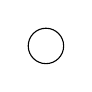
\begin{tikzpicture}[scale=0.5]
\draw (0,0) circle [radius=0.45];
\end{tikzpicture}
\else
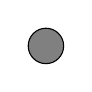
\begin{tikzpicture}[scale=0.5]
\draw [fill=gray] (0,0) circle [radius=0.45];
\end{tikzpicture}
\fi
\else
\begin{tikzpicture}[scale=0.5]
 \draw (0,0) circle [radius=0.45];
 \foreach \x in {0,...,#1}
  \draw [fill=gray] (0,0) -- (90:0.45) arc (90:90+\x*(360/#2):0.45) -- cycle;
 \foreach \x in {1,...,#2}
 \draw (0,0) -- (90:0.45) arc (90:90+\x*(360/#2):0.45) -- cycle;
\end{tikzpicture}
 \fi
}

\newcommand{\tsign}[1]{
\begin{tikzpicture}[scale=0.3]
 \draw [draw=white] (0,0) circle [radius=0.1] node {#1};
\end{tikzpicture}
}

     \newcommand{\winkel}[6][black]{
     \path[name path=circle] #3 circle [radius=#6 mm];
     \draw
     #2 coordinate (P1) -- 
     #3 coordinate (P2) -- 
     #4 coordinate (P3)
     pic[draw=#1,angle radius=#6 mm]
     {angle=P1--P2--P3};
     
     \path[
     name path=one
     ] (P1) -- (P2);
     \path[
     name path=two
     ] (P3) -- (P2);
     
     \path[
     name intersections={of=circle and one,by={W1}},
     name intersections={of=circle and two,by={W2}}
     ] (W1) -- (W2) coordinate[midway] (M);
     
     \node at ($#3!.7!(M)$) {#5};
     }


 \newcommand\gerade[6]{% 
  \coordinate (Punkt1) at (#1,#2); 
  \coordinate (Punkt2) at (#3,#4); 
  \pgfmathsetmacro\m{(#4-#2)/(#3-#1)}% 
  \pgfmathsetmacro\n{#2-\m*#1}% 
  \draw plot[domain=#5:#6] (\x,{\m*\x+\n}); 
} 
 
%Stromkreis-Symbole
\usetikzlibrary{
circuits.logic.US,
circuits.logic.IEC,
circuits.logic.CDH,
circuits.ee.IEC,
}

%Voltmeter
\tikzset{circuit declare symbol = voltmeter}
\tikzset{set voltmeter graphic ={draw,generic circle IEC, minimum size=5mm,info=center:V}}

%Amperemeter
\tikzset{circuit declare symbol = ammeter}
\tikzset{set ammeter graphic ={draw,generic circle IEC, minimum size=5mm,info=center:A}}

%variertes Voltmeter
\tikzset{circuit declare symbol = var voltmeter}
\tikzset{set var voltmeter graphic ={draw,generic circle IEC, minimum size=5mm,info=center:U}}

%variertes Amperemeter:
\tikzset{circuit declare symbol = var ammeter}
\tikzset{set var ammeter graphic ={draw,generic circle IEC, minimum size=5mm,info=center:$\mathtt{I}$}}

%AC Voltmeter
\tikzset{circuit declare symbol = AC voltmeter}
\tikzset{set AC voltmeter graphic ={draw,generic circle IEC, minimum size=6mm,info=center:{$\underset{\mathbf{\sim}}{\mathsf{V}}$}}}

%DC Voltmeter
\tikzset{circuit declare symbol = DC voltmeter}
\tikzset{set DC voltmeter graphic ={draw,generic circle IEC, minimum size=6mm,info=center:{$\underset{\mathbf{-}}{\mathsf{V}}$}}}

%ACDC Voltmeter
\tikzset{circuit declare symbol = ACDC voltmeter}
\tikzset{set ACDC voltmeter graphic ={draw,generic circle IEC, minimum size=6mm,info=center:{$\underset{\mathbf{\eqsim}}{\mathsf{V}}$}}}

%Einstellbare Widerstände
\tikzset{rough/.style={annotation arrow/.style = {> = *}}}
\tikzset{var rough/.style={annotation arrow/.style = {> = o}}}
\tikzset{stepped/.style={annotation arrow/.style = {> = |}}}
\tikzset{blank/.style={annotation arrow/.style = {> = none}}}

%%%%%%%%%%%%%%%%%%%%%%%%%%%%%%%%%%%%%%%%%%%%%%%%%%%%%%%%%%%%%%%%%%%%%%%%%%%%%%%%%%%%%%%%%%%%%%%%%%%%%%%%%%%%%%%%%%%%%%%%%%%%%%%%%%%%%%%%%%%%%%%%%%%%%%%%

\newcommand{\zirkelschnitt}[2]{
\begin{scope}
 \clip #2 circle [radius=0.5cm];
 \draw let 
 \p1 = #2,
 \p2 = #1,
 \n1 = {veclen((\x2-\x1),(\y2-\y1))}
 in
 #1 circle [radius=\n1];
 \end{scope}
}

\newcommand{\laenge}[2]{%#1=Mittelpunkt1, #2=Radius1, #3=Mittelpunkt2, #4=Radius2, #5=Schnittpunkt1,#6=Schnittpunkt2 
 let 
 \p1 = #2,
 \p2 = #1,
 \n1 = {veclen((\x2-\x1),(\y2-\y1))}
 in
}

\newcommand{\dreieck}[5]{
\begin{scope}
 \clip #1 -- #2;
 \path [name path=circle#1] #1 circle [radius=#3 cm];
 \path [name path=circle#2] #2 circle [radius=#4 cm];
 \path [name intersections={of={circle#1 and circle#2}}];
\end{scope}
\ifnum #5=2{
\coordinate (C) at (intersection-2);
}
\else
\coordinate (C) at (intersection-1);
\fi
}

\newcommand{\mittelpunkt}[2]{
\begin{scope}
\clip #1 -- #2;

\path [name path = linie12] #1 -- #2;

 \path let 
 \p1 = #1,
 \p2 = #2,
 \n1 = {veclen((\x2-\x1),(\y2-\y1))}
 in
[name path = circle1] #1 circle [radius=\n1];
\path let 
 \p1 = #1,
 \p2 = #2,
 \n1 = {veclen((\x2-\x1),(\y2-\y1))}
 in
[name path = circle2] #2 circle [radius=\n1];

\path [name intersections={of={circle1 and circle2}}];
\coordinate (H1) at (intersection-1);
\coordinate (H2) at (intersection-2);
\path [name path = hilfslinie] (H1) -- (H2);

\path [name intersections={of={linie12 and hilfslinie}}];
\coordinate (M) at (intersection-1);
\end{scope}
}

\newcommand{\thaleskreis}[3][]{
\mittelpunkt{#2}{#3}


 \clip let
 \p1 = #2,
 \p2 = (M),
 \n1 = {veclen((\x2-\x1),(\y2-\y1))}
 in 
 (\x1,\y1) rectangle ($#3+(0,\n1)$);

\draw let
\p1 = #2,
\p2 = (M),
\n1 = {veclen((\x2-\x1),(\y2-\y1))}
in
[#1,name path=thaleskreis] (M) circle [radius=\n1];
}


\newcommand{\BIn}[1]{
\def\r{1.5mm}
\draw (#1) circle (\r);	
\draw (#1) ++(45:\r) -- ++(180+45:2*\r);
\draw (#1) ++(90+45:\r) -- ++(360-45:2*\r);
}

\newcommand{\BOut}[1]{
\def\r{1.5mm}
\draw (#1) circle (\r);	
\draw[fill=black] (#1) circle (0.15mm);
}

%%%%%%%%%%%%%%%%%%%%%%%%%%%%%%%%%%%% Quader %%%%%%%%%%%%%%%%%%%%%%%%%%%%%%%%%%

\usetikzlibrary{3d}

\makeatletter
\def\tikz@lib@cuboid@get#1{\pgfkeysvalueof{/tikz/cuboid/#1}}

\def\tikz@lib@cuboid@setup{%
   \pgfmathsetlengthmacro{\vxx}%
      {\tikz@lib@cuboid@get{xscale}*cos(\tikz@lib@cuboid@get{xangle})*1cm}
   \pgfmathsetlengthmacro{\vxy}%
      {\tikz@lib@cuboid@get{xscale}*sin(\tikz@lib@cuboid@get{xangle})*1cm}
   \pgfmathsetlengthmacro{\vyx}%
      {\tikz@lib@cuboid@get{yscale}*cos(\tikz@lib@cuboid@get{yangle})*1cm}
   \pgfmathsetlengthmacro{\vyy}%
      {\tikz@lib@cuboid@get{yscale}*sin(\tikz@lib@cuboid@get{yangle})*1cm}
   \pgfmathsetlengthmacro{\vzx}%
      {\tikz@lib@cuboid@get{zscale}*cos(\tikz@lib@cuboid@get{zangle})*1cm}
   \pgfmathsetlengthmacro{\vzy}%
      {\tikz@lib@cuboid@get{zscale}*sin(\tikz@lib@cuboid@get{zangle})*1cm}
}

\def\tikz@lib@cuboid@draw#1--#2--#3\pgf@stop{%
    \begin{scope}[join=bevel,x={(\vxx,\vxy)},y={(\vyx,\vyy)},z={(\vzx,\vzy)}]
       % first fill the faces with global and individual style
       % then draw the grids
       \begin{scope}[canvas is yz plane at x=#1]
          \draw[cuboid/all faces,cuboid/edges,cuboid/right face] 
                (0,0) -- ++(#2,0) -- ++(0,-#3) -- ++(-#2,0) -- cycle;
          \draw[cuboid/all grids,cuboid/right grid] (0,0) grid (#2,-#3);
       \end{scope}
       \begin{scope}[canvas is xy plane at z=0]
          \draw[cuboid/all faces,cuboid/edges,cuboid/front face] 
                (0,0) -- ++(#1,0) --  ++(0,#2) -- ++(-#1,0) -- cycle;
          \draw[cuboid/all grids,cuboid/front grid] (0,0) grid (#1,#2);
       \end{scope}
       \begin{scope}[canvas is xz plane at y=#2]
          \draw[cuboid/all faces,cuboid/edges,cuboid/top face] 
                (0,0) -- ++(#1,0) --  ++(0,-#3) -- ++(-#1,0) -- cycle;
          \draw[cuboid/all grids,cuboid/top grid] (0,0) grid (#1,-#3);
       \end{scope}
       % now, draw the hidden edges
       \draw[cuboid/hidden edges] (0,#2,-#3) -- (0,0,-#3) -- (0,0,0) 
                (0,0,-#3) -- ++(#1,0,0);
       % finally, draw the visible edges 
       \begin{scope}[canvas is yz plane at x=#1]
          \draw[cuboid/all faces,cuboid/right face,cuboid/edges,fill opacity=0] 
                (0,0) -- ++(#2,0) -- ++(0,-#3) -- ++(-#2,0) -- cycle;
       \end{scope}
       \begin{scope}[canvas is xy plane at z=0]
          \draw[cuboid/all faces,cuboid/front face,cuboid/edges,fill opacity=0] 
                (0,0) -- ++(#1,0) --  ++(0,#2) -- ++(-#1,0) -- cycle;
       \end{scope}
       \begin{scope}[canvas is xz plane at y=#2]
          \draw[cuboid/all faces,cuboid/top face,cuboid/edges,fill opacity=0] 
                (0,0) -- ++(#1,0) --  ++(0,-#3) -- ++(-#1,0) -- cycle;
       \end{scope}
       % define the anchors: 8 vertices
       \path (0,#2,0) coordinate (-left top front)
                      coordinate (-left front top)
                      coordinate (-top left front)
                      coordinate (-top front left)
                      coordinate (-front top left)
                      coordinate (-front left top);
       \path (0,#2,-#3) coordinate (-left top rear)
                        coordinate (-left rear top)
                        coordinate (-top left rear)
                        coordinate (-top rear left)
                        coordinate (-rear top left)
                        coordinate (-rear left top);
       \path (0,0,-#3) coordinate (-left bottom rear)
                       coordinate (-left rear bottom)
                       coordinate (-bottom left rear)
                       coordinate (-bottom rear left)
                       coordinate (-rear bottom left)
                       coordinate (-rear left bottom);
       \path (0,0,0) coordinate (-left bottom front)
                     coordinate (-left front bottom)
                     coordinate (-bottom left front)
                     coordinate (-bottom front left)
                     coordinate (-front bottom left)
                     coordinate (-front left bottom);
       \path (#1,#2,0) coordinate (-right top front)
                       coordinate (-right front top)
                       coordinate (-top right front)
                       coordinate (-top front right)
                       coordinate (-front top right)
                       coordinate (-front right top);
       \path (#1,#2,-#3) coordinate (-right top rear)
                         coordinate (-right rear top)
                         coordinate (-top right rear)
                         coordinate (-top rear right)
                         coordinate (-rear top right)
                         coordinate (-rear right top);
       \path (#1,0,-#3) coordinate (-right bottom rear)
                        coordinate (-right rear bottom)
                        coordinate (-bottom right rear)
                        coordinate (-bottom rear right)
                        coordinate (-rear bottom right)
                        coordinate (-rear right bottom);
       \path (#1,0,0) coordinate (-right bottom front)
                      coordinate (-right front bottom)
                      coordinate (-bottom right front)
                      coordinate (-bottom front right)
                      coordinate (-front bottom right)
                      coordinate (-front right bottom);
       % centers of the 6 faces
       \coordinate (-left center) at (0,.5*#2,-.5*#3);
       \coordinate (-right center) at (#1,.5*#2,-.5*#3);
       \coordinate (-top center) at (.5*#1,#2,-.5*#3);
       \coordinate (-bottom center) at (.5*#1,0,-.5*#3);
       \coordinate (-front center) at (.5*#1,.5*#2,0);
       \coordinate (-rear center) at (.5*#1,.5*#2,-#3);
       % center of the cuboid
       \coordinate (-center) at (.5*#1,.5*#2,-.5*#3);
       % centers of the 12 edges
       \path (0,#2,-.5*#3) coordinate (-left top center) 
                           coordinate (-top left center);
       \path (.5*#1,#2,-#3) coordinate (-top rear center)
                            coordinate (-rear top center);
       \path (#1,#2,-.5*#3) coordinate (-right top center)
                            coordinate (-top right center);
       \path (.5*#1,#2,0) coordinate (-top front center)
                          coordinate (-front top center);
       \path (0,0,-.5*#3) coordinate (-left bottom center) 
                           coordinate (-bottom left center);
       \path (.5*#1,0,-#3) coordinate (-bottom rear center)
                            coordinate (-rear bottom center);
       \path (#1,0,-.5*#3) coordinate (-right bottom center)
                            coordinate (-bottom right center);
       \path (.5*#1,0,0) coordinate (-bottom front center)
                          coordinate (-front bottom center);
       \path (0,.5*#2,0) coordinate (-left front center) 
                           coordinate (-front left center);
       \path (0,.5*#2,-#3) coordinate (-left rear center)
                            coordinate (-rear left center);
       \path (#1,.5*#2,0) coordinate (-right front center)
                            coordinate (-front right center);
       \path (#1,.5*#2,-#3) coordinate (-right rear center)
                          coordinate (-rear right center);
    \end{scope}
}

\tikzset{
  pics/cuboid/.style = {
    setup code = \tikz@lib@cuboid@setup,
    background code = \tikz@lib@cuboid@draw#1\pgf@stop
  },
  pics/cuboid/.default={1--1--1},
  cuboid/.is family,
  cuboid,
  all faces/.style={fill=white},
  all grids/.style={draw=none},
  front face/.style={},
  front grid/.style={},
  right face/.style={},
  right grid/.style={},
  top face/.style={},
  top grid/.style={},
  edges/.style={},
  hidden edges/.style={draw=none},
  xangle/.initial=0,
  yangle/.initial=90,
  zangle/.initial=210,
  xscale/.initial=1,
  yscale/.initial=1,
  zscale/.initial=0.5
}

\newcommand{\tikzcuboidreset}{
\tikzset{cuboid,
  all faces/.style={fill=white},
  all grids/.style={draw=none},
  front face/.style={},
  front grid/.style={},
  right face/.style={},
  right grid/.style={},
  top face/.style={},
  top grid/.style={},
  edges/.style={},
  hidden edges/.style={draw=none},
  xangle=0,
  yangle=90,
  zangle=210,
  xscale=1,
  yscale=1,
  zscale=0.5
}
}

\newcommand*\circled[1]{\tikz[baseline=(char.base)]{
            \node[shape=circle,draw,inner sep=2pt] (char) {#1};}}


\newcommand{\tikzcuboidset}{\@ifstar\tikzcuboidset@star\tikzcuboidset@nostar} 
\newcommand{\tikzcuboidset@nostar}[1]{\tikzcuboidreset\tikzset{cuboid,#1}}
\newcommand{\tikzcuboidset@star}[1]{\tikzset{cuboid,#1}}
\makeatother


